\documentclass[11pt]{article}
\usepackage{fullpage}
\usepackage{hyperref}
\usepackage{amsmath}
\usepackage{graphicx}
\usepackage{parskip}
\usepackage{mutlirow}

\begin{document}
\title{Predicting the Outcome of Soccer Matches}
\author{Ayaan Kazerouni and Harsh Patel}
\date{}
\maketitle

\section{Problem Statement}
Soccer is a widely played sport, and is arguably the only globally played sport.
We thought it would be interesting to develop a model that could predict the winner of a soccer game, a task called the `holy grail' by the provider of the dataset. Our problem statement is formally defined as follows:

We have access to a dataset that has featrures from matches already played, ranging from the number of goals scored by home team and away team to different attributes of the players of individual teams. Given this dataset, our goal is to build a model that predicts the winner of the match fairly accurately.
As with a lot of parameters in data analytics and machine learning, `fairly accurately' is a vague term, but we define it as anything better than 53\%, which is the accuracy achieved by the dataset provider (and the target accuracy we mentioned in our proposal).
We are unaware of the features used in their model or the nature of their model. We have also not looked at what others have done with this dataset.
The work presented in this report is solely our own.

\section{Data Description}
\label{sec:data-desc}
We have chosen a European soccer dataset~\cite{mathien1}, the nature of which as described by the provider is:
\begin{itemize}
  \setlength\itemsep{0em}
  \item{+25,000 matches}
  \item{+10,000 playres}
  \item{11 European countries with their lead championship}
  \item{Seasons 2008 to 2016}
  \item{Players and Teams' attributes sourced from EA Sports' FIFA video game series, including the weekly updates}
  \item{Team line up with squad formation (X, Y coordinates)}
  \item{Betting odds from up to 10 providers}
  \item{Detailed match events (goal types, possession, corner, cross, fouls, cards etc...) for +10,000 matches}
\end{itemize}
We are thankful to the data provider for consolidating and organizing the data from various online sources.
This has reduced work on finding relevant data on our part considerably.

The data is provided in a relational database (SQLite3) of \textit{Matches}, \textit{Players}, \textit{Player-Attributes}, \textit{Teams}, \textit{Team-Attributes}, \textit{Leagues}, and \textit{Countries}.
A description of the magnitude of the data is provided in Table~\ref{tab:data-desc}.

\begin{table}[ht]
\centering
\begin{tabular}{|l|r|r|}
\hline
\textbf{}                   & \textbf{Count} & \textbf{Dimensions} \\ \hline
\textbf{Match}              & 25979          & 115                 \\ \hline
\textbf{Teams}              & 299            & 5                   \\ \hline
\textbf{Team\_Attributes}   & 1458           & 25                  \\ \hline
\textbf{Player}             & 11060          & 7                   \\ \hline
\textbf{Player\_Attributes} & 183978         & 42                  \\ \hline
\textbf{Country}            & 11             & 2                   \\ \hline
\textbf{League}             & 11             & 3                   \\ \hline
\end{tabular}
\caption{Magnitude of the available data}
\label{tab:data-desc}
\end{table}

Here, the active reader would have noticed that there are only 299 teams but 1458 Team\_Attribute rows.
This is because the data provider has provided the attributes for some teams over a span of several years and intuitively enough, the attributes keep changing over time.
The same is true for the player attributes.

Some descriptive statistics for team attributes can be seen in table~\ref{tab:desc-stat}.

\begin{table}[ht]
\centering
\begin{tabular}{rllllll}
  \hline
                 & Min     & 1st Qu. & Median  & Mean    & 3rd Qu. & Max \\
  \hline
buildUpPlaySpeed & 20.00   & 45.00   & 52.00   & 52.46   & 62.00   & 80.00   \\
  buildUpPlayPassing & 20.00   & 40.00   & 50.00   & 48.49   & 55.00   & 80.00   \\
  chanceCreationPassing & 21.00   & 46.00   & 52.00   & 52.17   & 59.00   & 80.00   \\
  chanceCreationCrossing & 20.00   & 47.00   & 53.00   & 53.73   & 62.00   & 80.00   \\
  chanceCreationShooting & 22.00   & 48.00   & 53.00   & 53.97   & 61.00   & 80.00   \\
  defencePressure & 23.00   & 39.00   & 45.00   & 46.02   & 51.00   & 72.00   \\
  defenceAggression & 24.00   & 44.00   & 48.00   & 49.25   & 55.00   & 72.00   \\
  defenceTeamWidth & 29.00   & 47.00   & 52.00   & 52.19   & 58.00   & 73.00   \\
   \hline
\end{tabular}
\caption{5-number summaries for team attributes}
\label{tab:desc-stat}
\end{table}

\subsection{Data Exploration}
With our objective in mind, the following two tables were of interest to us:
\begin{itemize}
  \setlength\itemsep{0em}
  \item Match
  \item Team\_Attributes
\end{itemize}
Although, Player\_Attributes might give useful information about the strengths of the team, we haven't delved much into it as there are numerous attributes of the players and for each match, we would have to come up with a normalized attribute for the whole team. This would complicate our model and we aimed at keeping the model as simple as possible to avoid overfitting.

From the structure of the data, it is apparent that the rest of the tables, except player attributes, are used for indexing purposes (eg. foreign keys from leagues to countries).
These data entries, being nominal attributes, are just used to differentiate between two different entities and hence do not contribute towards finding out interesting patterns in the data.

\subsection{K-means Clustering}
K-Means clustering on team attributes provided some interesting insights.
First, we needed to pick a value for $k$.
To do this, we followed~\cite{cluster1}.
We performed k-means clustering for different values of $k$ from 2 to 12, and plotted the SSE for each $k$.
Our dataset had $n = ~25000$, so this process was relatively inexpensive in R.
The decrease in SSE from 2 to 3 was large but didn't change as much past that.
This told us that $k=3$ was an optimum number of clusters.
The plot is in figure~\ref{fig:sse}.

\begin{figure}[ht!]
  \centering
  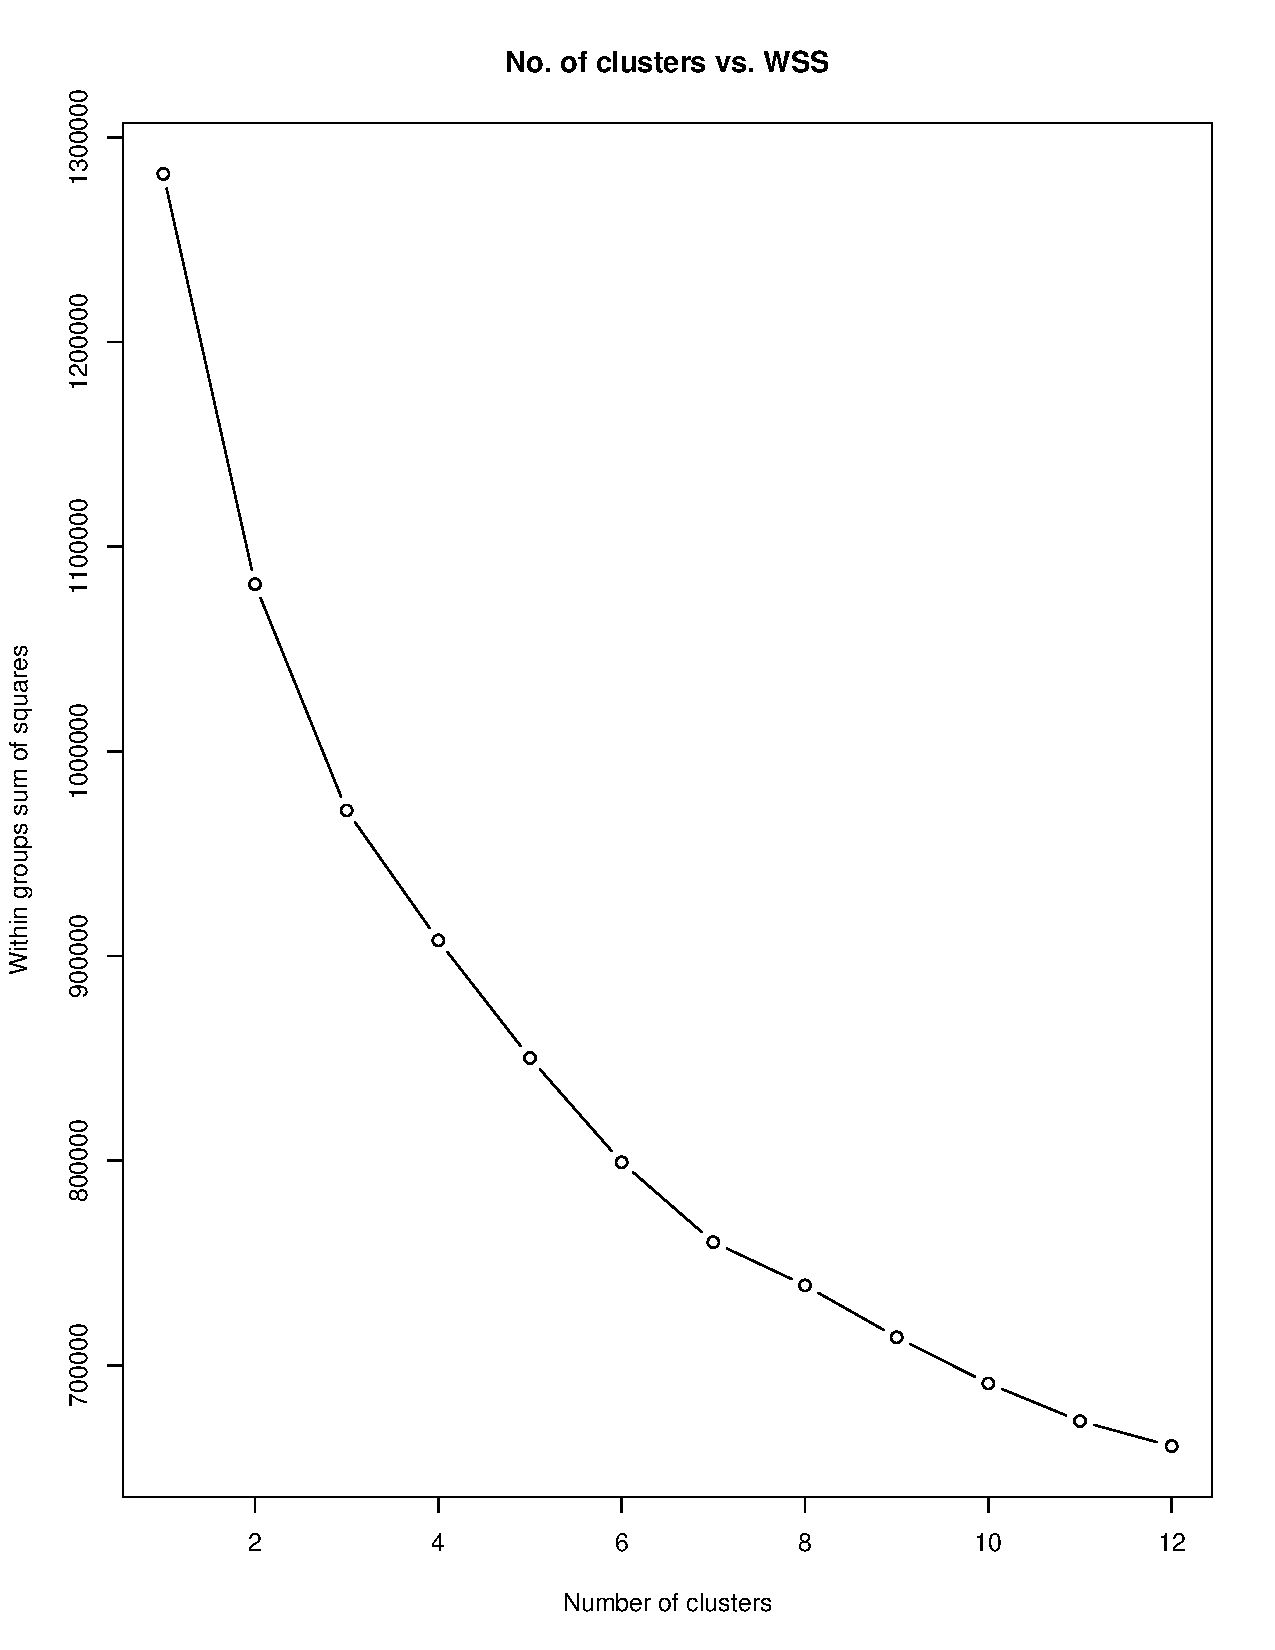
\includegraphics[scale=0.5]{wss}
  \caption{Decrease in SSE as k increases.}
  \label{fig:sse}
\end{figure}

Once we had selected $k$, we performed k-means clustering on the team attributes for each year in 2010 to 2015.
To visualize the clustered team attributes, we performed Principlal Component Analysis (PCA) to reduce the dimensionality from 8 to 2.
The PCA-reduced clusters are in figure~\ref{fig:clusters}.
We can see more variability between teams in 2010 than in subsequent years.
In other words, given two teams, it would be easier to categorize them in 2010 -- which presumably means that it would be easier to determine the outcome between two teams in different clusters.
For years 2011, the clusters are denser and closer together for the most part, indicating that teams were more closely matched up in 2011.
The remaining years see the teams moving further apart again, but not as much as 2010.

\textbf{Please note that the clustering took place on the original data.
PCA was used for visualization purposes only.}

\begin{figure}[ht]
  \centering
  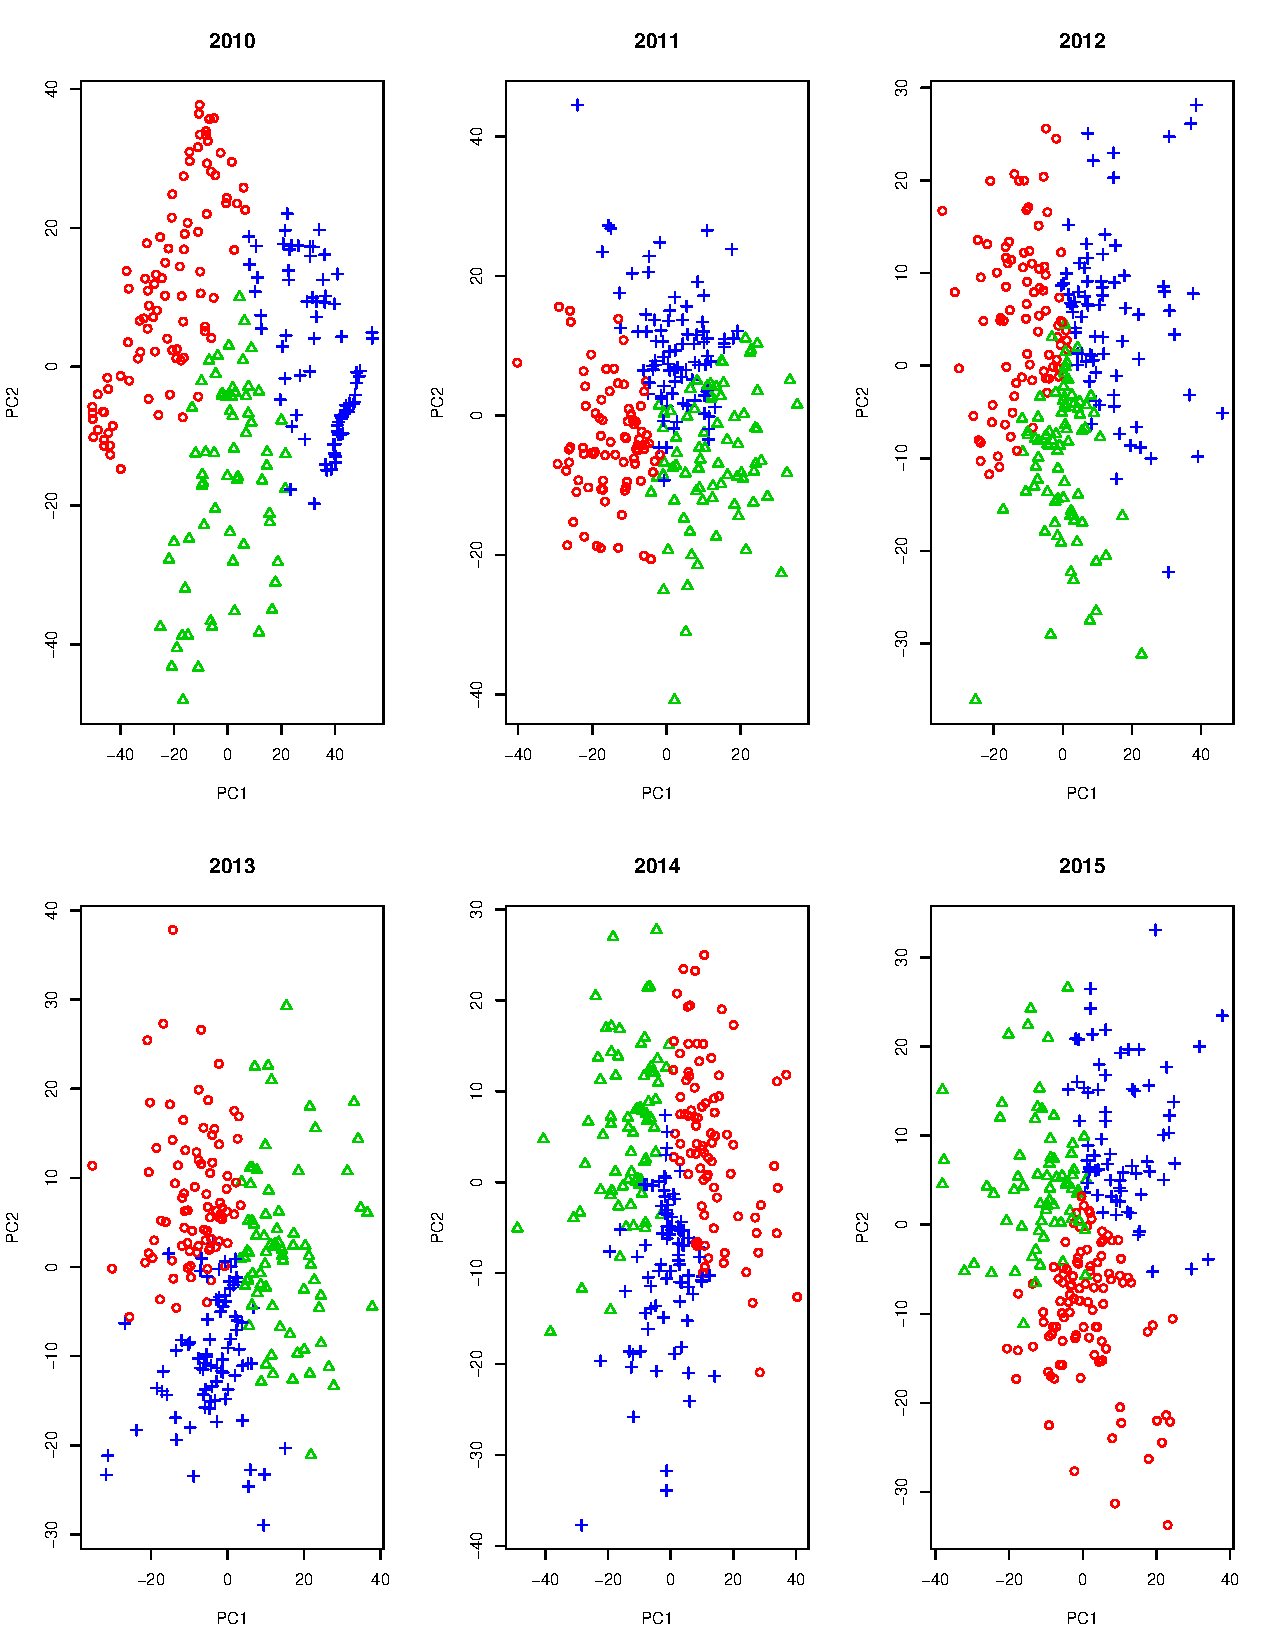
\includegraphics[scale=0.6]{clusters}
  \caption{PCA-reduced clustered team attributes for 6 years.}
  \label{fig:clusters}
\end{figure}

\subsection{Data Preprocessing}
\label{sec:preprocessing}
Looking at Table~\ref{tab:data-desc} again, notice that Match and Team\_Attributes have 115 and 25 attributes, respectively.
The Match table contained the following relevant dimensions:
\begin{itemize}
  \setlength\itemsep{0em}
  \item season
  \item stage
  \item date
  \item home\_team\_id
  \item away\_team\_id
  \item home\_team\_goal
  \item away\_team\_goal
  \item goal
  \item shoton
  \item shotoff
  \item cross
  \item corner
  \item possession
\end{itemize}
\noindent
The Team Attributes provided were the following:
\begin{itemize}
  \setlength \itemsep{0em}
  \item buildUpPlaySpeed
  \item buildUpPlayPassing
  \item chanceCreationPassing
  \item chanceCreationCrossing
  \item chanceCreationShooting
  \item defencePressure
  \item defenceAggression
  \item defenceTeamWidth
\end{itemize}

All the above listed attributes are continuous.
In addition to them, the database also contained a discretized value for each attribute listed above.
For the preprocessing methodology we describe below, it was necessary to choose the continuous versions of these attributes.
Also, there existed an attribute called \textit{buildUpPlayDribbling} that was not present in 969 (66\%) Team\_Attribute rows.
This is a large percentage, and in addition to that, discarding rows with this NULL value would have had a ripple effect, causing us to discard too many matches.

Since the data was provided as a relational database, significant pre-processing steps were undertaken before modelling began.

Here, instead of tranforming the data to a new space using techniques such as Principal Component Analysis (PCA) or Multimdimensional Scaling (MDS), we have kept the data in its original state and used domain specific knowledge to hand pick some interesting features.
Handpicking the features we have reduced the dimensionality complexity from 115 to a little more than 10.

\subsection{Difference Vectors}
During our ideation phase, we realized that when two teams are facing each other, we would need a method with which to compare the two teams.
The simplest method to do this was to calculate a `difference vector' for each match -- a vector of the differences between each involved team's attributes.

The next question that arose was how to identify \textit{which} team we were making a prediction about.
Our solution was to change the problem from \textbf{Predicting the winner} to \textbf{Predicting the result for the home team}.
Doing things this way fell in line nicely for our concept of `difference vectors'.
If $h$ is a vector of the home team's attributes and $a$ is a vector of the away team's attributes, then $d = h - a$, where $d$ is the difference vector, \textit{from the perspective of the home team}.

For example, see the home team $h$, the away team $a$, and their difference vector presented in table~\ref{tab:diff}.
The vector $d = h - a$ for each match is what is passed to our models for prediction.

\begin{table}[ht]
\centering
\begin{tabular}{|l|c|c|c|}
\hline
                                & \textbf{h} & \textbf{a} & \textbf{d = h - a} \\ \hline
\textbf{buildUpPlaySpeed}       & 61         & 50         & 11             \\ \hline
\textbf{buildUpPlayPassing}     & 46         & 54         & -8             \\ \hline
\textbf{chanceCreationPassing}  & 66         & 52         & 14             \\ \hline
\textbf{chanceCreationCrossing} & 66         & 54         & 12             \\ \hline
\textbf{chanceCreationShooting} & 54         & 46         & 8              \\ \hline
\textbf{defencePressure}        & 47         & 36         & 11             \\ \hline
\textbf{defenceAggression}      & 58         & 43         & 15             \\ \hline
\textbf{defenceTeamWidth}       & 53         & 47         & 6              \\ \hline
\end{tabular}
\caption{Difference vector}
\label{tab:diff}
\end{table}

\subsubsection{Which attributes to use?}
As mentioned in Section~\ref{sec:data-desc}, each team had several vectors of attributes associated with it, since they had potentially differing attributes each year.
As can be seen in figure~\ref{fig:clusters}, the distributions of team attributes were not static across the 6 years for which team information is available.
As a result, for a particular team playing a particular match, we used the vector of attributes with the date \textit{closest to the match date}.
This typically meant we used attributes from the same sporting season.

\subsubsection{Defining the outcome variable}
Recall that, for each match, the database provided a home\_goal count and an away\_goal count.
Since we had turned our problem into a prediction for the home team, we defined an $outcome$ categorical variable for each difference vector.
The variable has 3 levels: 0 if the home team lost, 1 if the match was a draw, and 2 if the home team won.

We also defined a $win\_percentage$ variable that looked at past encounters between two given teams.
This variable will be discussed in further detail in Section~\ref{sec:models}.

\section{Prediction Algorithms}
We started by predicting if the home would \textit{win} or \textit{not win}.
Hence, we changed the outcome of the match from 0 (lose), 1 (draw), and 2 (win) to just 0 (lose or draw) and 1 (win).
After processing the data in a way that will be suitable for our intended task, we used various classification and regression models to come up with the outcome given two different teams and their respective attributes.
The algorithms we used are presented in this section.

\subsection{Decision Tree}
\textbf{Attributes Used:}
\begin{itemize}
  \setlength\itemsep{0em}
  \item buildUpPlaySpeed
  \item buildUpPlayPassing
  \item chanceCreationPassing
  \item chanceCreationCrossing
  \item chanceCreationShooting
  \item defencePressure
  \item defenceAggression
  \item defenceTeamWidth
\end{itemize}
\textbf{Decision Tree:}
Generated by THIS.\\
\textbf{Accuracy:} 50\%

Based on what we mentioned in our proposal, we initially implemented a decision tree classifier.
For the decision tree, we only used the attributes of the Difference Vector.
We trained the decision tree on 80\% of the data and used the remaining 20\% for testing.

Unfortunately, the decision tree did not perform particularly well.
We achieved approximately 50\% accuracy, which is essentially the accuracy of a random guess for a binary variable.
To improve these results, we decided to try another classification method.

\subsection{Logistic Regression}
We went through several versions of the logistic regression, makign strategic changes to the features involved each time. The details of each iteration are presented below.

\subsubsection{Iteration 1:}
The Match table contained betting odds as published by 10 bookkeeping companies.
The odds were presented as the odds of the home team winning (H), the odds of a draw (D), and the odds of the away team winning (A).
We added one company's odds to our featureset (for a total of 3 additional variables).
We trained a stepwise logistic regression using these features to predict 0 (lose or draw) or 1 (win).

Performing 5-fold cross validation, each time using 80\% as the training set and 20\% as the testing set, we achieved ~65\% accuracy.
This was encouraging, since it represented a 15\% jump from the accuracy achieved with a decision tree.
However, the Odds variables represented other professionals' predictions of the match outcome. 
Hence, we did not want to use these predictors in our predictor. Therefore, we decided to remove those from the model.

\subsubsection{Iteration 2:}
We re-ran the logistic regression model with the same difference vector (table~\ref{tab:diff}) as we used for the decision tree. The accuracy achieved by the logistic regression model was 54\%. The increase in accuracy from that of a decision tree is not significant in this case.

The confusion matrix for ~5000 test data entries is given by:
\begin{table}[]
\centering
\begin{tabular}{|l|l|r|r|}
\hline
\multicolumn{2}{|l|}{\multirow{2}{*}{}}                                     & \multicolumn{2}{l|}{Predicted class} \\ \cline{3-4} 
\multicolumn{2}{|l|}{}                                                      & 0                  & 1               \\ \hline
\multirow{2}{*}{\begin{tabular}[c]{@{}l@{}}Actual\\ Class\end{tabular}} & 0 & 2694               & 9               \\ \cline{2-4} 
                                                                        & 1 & 2410               & 13              \\ \hline
\end{tabular}
\caption{Logistic Regression Confusion Matrix}
\label{logistic-fusion1}
\end{table}
To include more meanigful attributes in our model, we came up with `Win Percentage' attribute for each team.
We define `Win Percentage' as follows:

Given two teams, we find all their past encounters. A clear win is treated as a win only, but to save ourselves from the curse of 0 in a multiplication, we treat a draw as a win by both teams instead of assigning a 0 to both teams.
\begin{align*}
win\_percentage\_team1 &= \frac{matches\;won\;by\;team1}{matches\;won\;by\;team1 + matches\;won\;by\;team2} \\
win\_percentage\_team2 &= \frac{matches\;won\;by\;team2}{matches\;won\;by\;team1 + matches\;won\;by\;team2}
\end{align*}
*Given that the data is provided for past 6 years, we are farily sure about a considerable number of encounters between any two teams. Hence, no matter which two teams are playing from given data, we will always come up with a non-zero win\_percentage for both teams. It is highly unlikely (for this dataset) to find a combination of a teams that haven't played each other in past.

\subsection{Binomial Regression}
First, we just tried to predict if home\_team wins or loses. We are not trying to predict the result as a 'draw'.
In this case home\_team\_win outcome is represented as a 1 and home\_team\_lose as a 0.
We use the same outcomes used for a decision tree.

\subsection{Multinomial Regression}
We tried to predict the outcome as a draw as well along with a win or lose, 



\bibliography{report.bib}
\bibliographystyle{plain}
\end{document}






